\documentclass[11pt,a4paper,onecolumn]{article}
\usepackage[left=3cm,right=3cm,top=2cm,bottom=2cm]{geometry}
\usepackage{amsmath}
\usepackage{float}
\usepackage{graphicx}
\DeclareGraphicsExtensions{.eps,.ps,.jpg,.bmp,.pdf}
\usepackage{ctex}
\usepackage{url}
\usepackage{listings}
\usepackage{color}
\definecolor{mygreen}{rgb}{0,0.6,0}
\definecolor{mygray}{rgb}{0.5,0.5,0.5}
\definecolor{mymauve}{rgb}{0.58,0,0.82}
\lstset{
	backgroundcolor=\color{white},
	basicstyle=\footnotesize,
	breakatwhitespace=false,
	breaklines=true,
	captionpos=b,
	commentstyle=\color{mygreen},
	deletekeywords={...},
	extendedchars=true,
	keepspaces=true,
	keywordstyle=\color{blue},
	language=R,
	otherkeywords={*,...},
	numbers=left,
	numbersep=5pt,
	numberstyle=\tiny\color{mygray},
	rulecolor=\color{black},
	showspaces=false,
	showstringspaces=false,
	showtabs=false,
	stepnumber=1,
	stringstyle=\color{mymauve},
	tabsize=2,
	}

\begin{document}
\title{\bfseries 探索性数据分析第一次作业 \\ \Large 使用ggplot2绘制中国地图}
\date{}
\author{黎思言 \\ 2016210669 \\ 2016应用统计专业硕士班}
\maketitle

\begin{abstract}
2016年,随着就业压力的增加和房价的不断攀升,工资水平和房价水平是毕业生在选择第一份工作所在的城市的时候考虑的两大因素。在中国34个省、自治区、直辖市和特别行政区中,哪些地区的工资水平最高,哪些地区的房价水平相对较低?这是本文研究的主要问题。本文从中经网上收集全国各省城镇居民家庭人均总收入、房地产开发企业商品房销售额和房地产开发企业商品房销售面积等数据分析发现:1.上海市、北京市、浙江省、江苏省、广东省为城镇居民人均可支配收入最高的五省市。甘肃省、黑龙江省、吉林省、贵州省、青海省为城镇居民人均可支配收入最低的五省。2.北京市、上海市、天津市、浙江省、广东省为房地产开发企业商品房销售平均价格最高的五省市。宁夏回族自治区、贵州省、内蒙古自治区、新疆维吾尔自治区、湖南省为房地产开发企业商品房销售平均价格最低的五省。3.相比较于人均可支配收入水平,北京市、上海市、天津市、广东省、海南省、湖北省、河北省、安徽省、四川省、江西省、陕西省、青海省、吉林省、黑龙江省、甘肃省、西藏自治区、山西省、河南省等省市房价偏高。浙江省、福建省、江苏省、辽宁省、山东省、重庆市、云南省、广西壮族自治区、湖南省、新疆维吾尔族自治区、内蒙古自治区、贵州省、宁夏回族自治区等省市房价相对较低。在本文最后一节,我使用shiny和plotly将上述三个图形做成了交互式app。
\end{abstract}

\section{收集数据}

\subsection{地图数据}

(1)从互联网中下载中国分省市的shp格式地图数据。地图地址:\url{http://muchong.com/html/201304/5748467.html};

(2)使用maptools包读取该地图文件,并将地图数据中的地名全部转化成utf8格式编码;

(3)使用ggplot2中的fortify函数将地图数据转换成gglot2方便处理的data.frame格式,并增加一列表示各省市的名称;

(4)获取各省市省会城市的地理坐标;我想要在地图的省会城市上标注该省的名称,所以应该获取各省市省会城市的地理坐标。我先从互联网上获取了全国34个省、自治区、直辖市和特别行政区的名称以及省会城市名称,然后使用腾讯地图开放平台的API获取了这些地区的坐标。

\subsection{填充数据}

我从中经网上下载了 城镇居民家庭人均总收入\_可支配收入\_累计.xls 房地产开发企业商品房销售额\_累计.xls 房地产开发企业商品房销售面积\_累计.xls 等三个数据表。可支配收入表包含了从2015年一季度到2016年四季度全国31个省、自治区和直辖市每个季度的城镇居民年累计人均可支配收入值,单位元。商品房销售额表包含了从2015年1月到2016年12月,全国31个省、自治区和直辖市每个月年累计商品房销售额,单位亿元。销售面积表包含了从2015年1月到2016年12月,全国31个省、自治区和直辖市每个月年累计商品房销售面积,单位万平方米。我将上述三表手动转化成csv格式之后读入R。

\section{绘制地图}

在本例中我使用的R包有ggplot2, showtext, grid, grDevices。

\subsection{2016年城镇居民家庭人均可支配收入}

\begin{figure}[H]
	\centering
	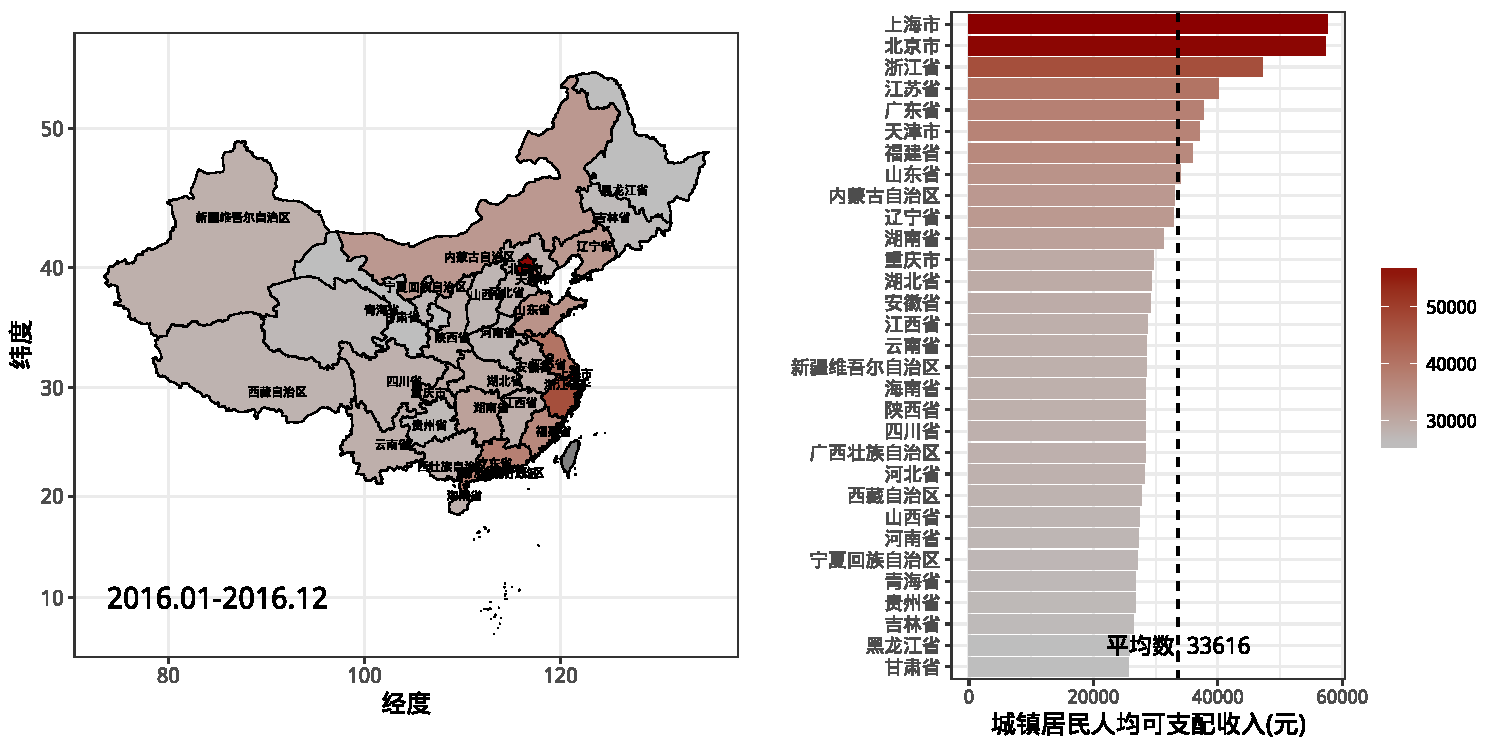
\includegraphics[width=400pt]{城镇居民人均可支配收入.pdf}
	\caption{2016年中国城镇居民人均可支配收入}
\end{figure}

从左图可知,2016年城镇具名家庭人均可支配收入呈现出东南沿海省市较高,中西部省市较低的特征。2016年,城镇居民人均可支配收入平均数为3.36万元。上海市、北京市、浙江省、江苏省、广东省为城镇居民人均可支配收入最高的五省市。甘肃省、黑龙江省、吉林省、贵州省、青海省为城镇居民人均可支配收入最低的五省。

\subsection{2016年房地产开发企业商品房销售平均价格}

\begin{figure}[H]
	\centering
	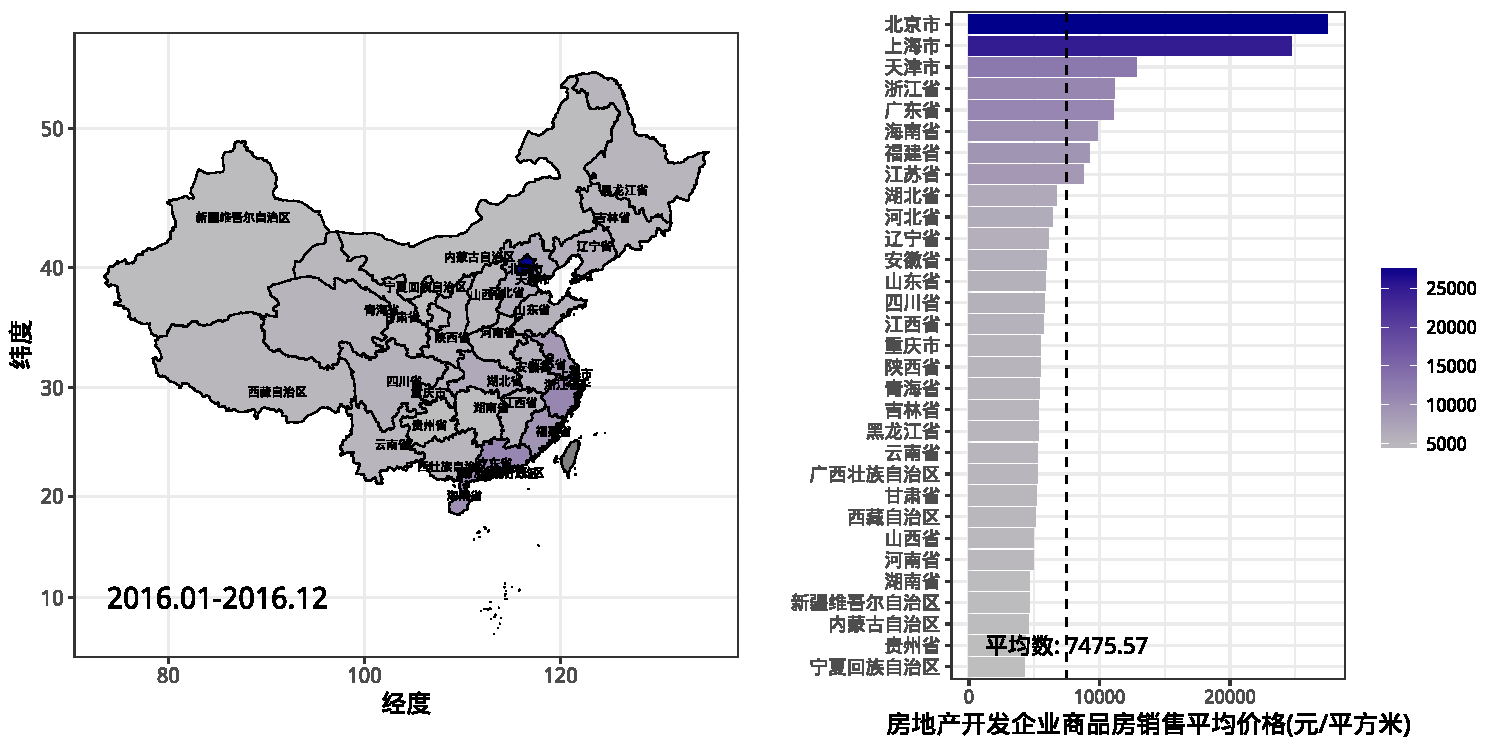
\includegraphics[width=400pt]{房地产开发企业商品房销售平均价格.pdf}
	\caption{2016年房地产开发企业商品房销售平均价格}
\end{figure}

房地产开发企业商品房销售平均价格等于房地产开发企业商品房销售额除以房地产开发企业商品房销售面积,单位元/平方米。从左图看出,2016年房地产开发企业商品房销售平均价格呈现出东部沿海省市较高,中西部省市较低的特征。2016年,房地产开发企业商品房销售平均价格平均数为每平方米7475元。北京市、上海市、天津市、浙江省、广东省为房地产开发企业商品房销售平均价格最高的五省市。宁夏回族自治区、贵州省、内蒙古自治区、新疆维吾尔自治区、湖南省为房地产开发企业商品房销售平均价格最低的五省。

\subsection{探索}

建立回归模型:
$$y_i = \beta_0 + \beta_1 x_i + \epsilon_i$$
$$\epsilon_i | x \sim N(0, \sigma^2)$$

其中$y$表示房地产开发企业商品房销售平均价格,$x$表示城镇居民家庭人均可支配收入,$\epsilon$是残差项。本例使用最小二乘估计参数。
$$\hat{\beta_1}=\frac{\sum(x_i-\bar{x})(y_i-\bar{y})}{\sum(x_i-\bar{x})^2}$$
$$\hat{\beta}_0=\bar{y}-\hat{\beta}_1\bar{x}$$
$$\hat{\epsilon}=y-\hat{y}$$

求出$R^2$:
$$R^2=\frac{\sum(\hat{y}_i-\bar{y})^2}{\sum(y_i-\bar{y})^2}$$

\begin{figure}[H]
	\centering
	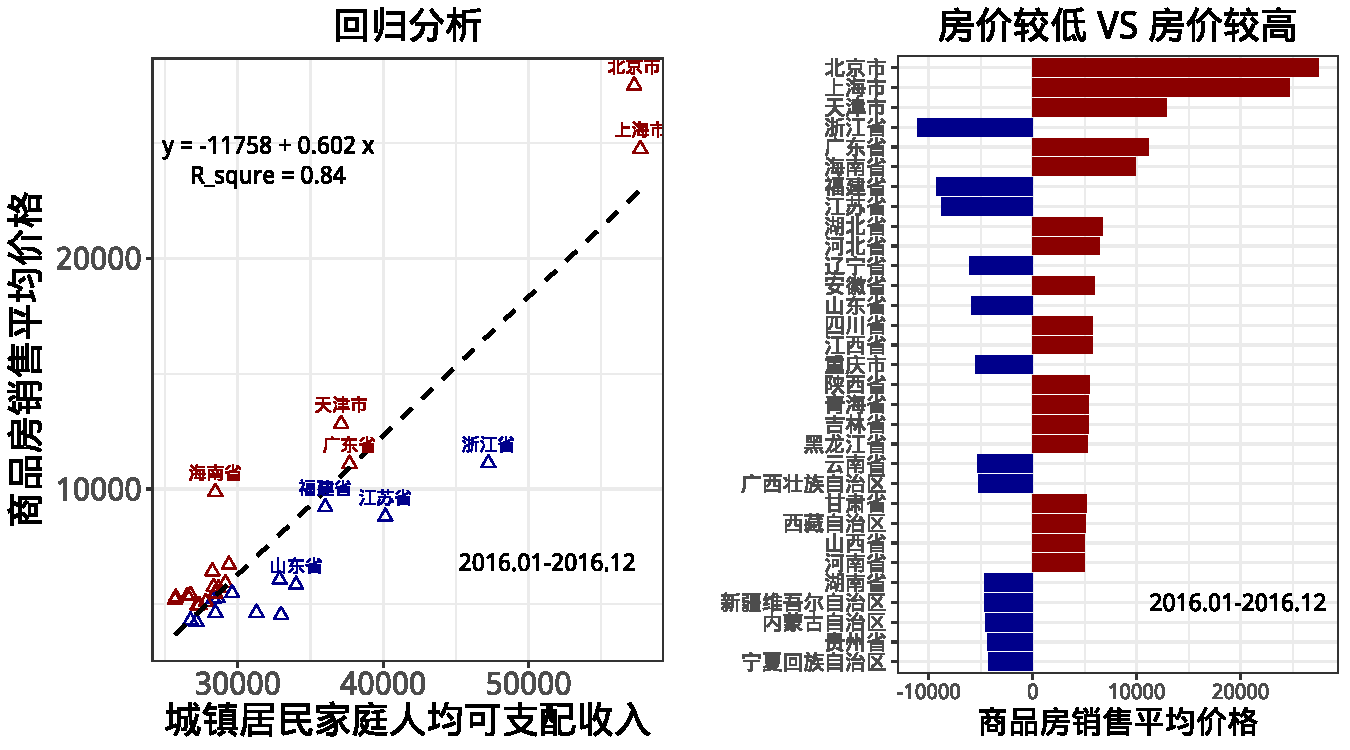
\includegraphics[width=400pt]{回归模型.pdf}
	\caption{2016年房地产开发企业商品房销售平均价格和城镇居民家庭人均可支配收入回归分析。左图横轴表示城镇居民家庭人均可支配收入,纵轴表示房地产开发企业商品房销售平均价格,时间区间是2016年全年,红点表示该省市房地产开发企业商品房销售平均价格高于回归直线,蓝点表示该省市房地产开发企业商品房销售平均价格低于回归直线。右图红色柱表示商品房销售平均价格高于回归直线省市的价格。蓝色柱表示商品房销售平均价格低于回归直线省市的价格。}
\end{figure}

从全国31个省、自治州和直辖市的数据建立回归模型发现,2016年,城镇居民家庭人均可支配收入每增加1元,房地产开发企业商品房销售平均价格上升0.602元/平方米。相比较于人均可支配收入水平,北京市、上海市、天津市、广东省、海南省、湖北省、河北省、安徽省、四川省、江西省、陕西省、青海省、吉林省、黑龙江省、甘肃省、西藏自治区、山西省、河南省等省市房价偏高。浙江省、福建省、江苏省、辽宁省、山东省、重庆市、云南省、广西壮族自治区、湖南省、新疆维吾尔族自治区、内蒙古自治区、贵州省、宁夏回族自治区等省市房价相对较低。

\section{shiny和plotly}

使用以下代码打开shinyapp.app。

\begin{lstlisting}
  library(shiny)
	runApp(./shinyapp)
\end{lstlisting}

打开app之后可以看到三个交互式图形,这三个图形分别是城镇居民家庭人均可支配收入地图、房地产开发企业商品房销售平均价格地图和散点图。在这三个图形的左边都配有菜单栏可调整相关参数。菜单栏可以选择图像展示的方式,支持在气泡图和地图中切换。菜单栏可以调整比较的时间段。鼠标悬停的位置会呈现该省市的城镇居民家庭人均可支配收入信息。图像可以放大或缩小。按住鼠标左键点选某区域之后可以将某区域信息放大。

\begin{figure}[H]
	\centering
	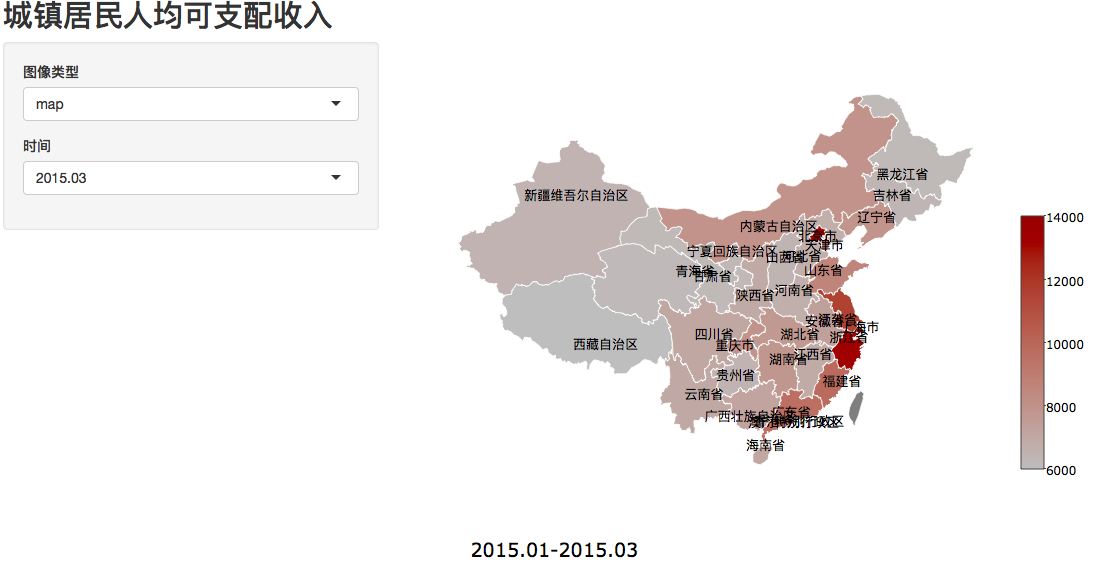
\includegraphics[width=400pt]{fig1.png}
	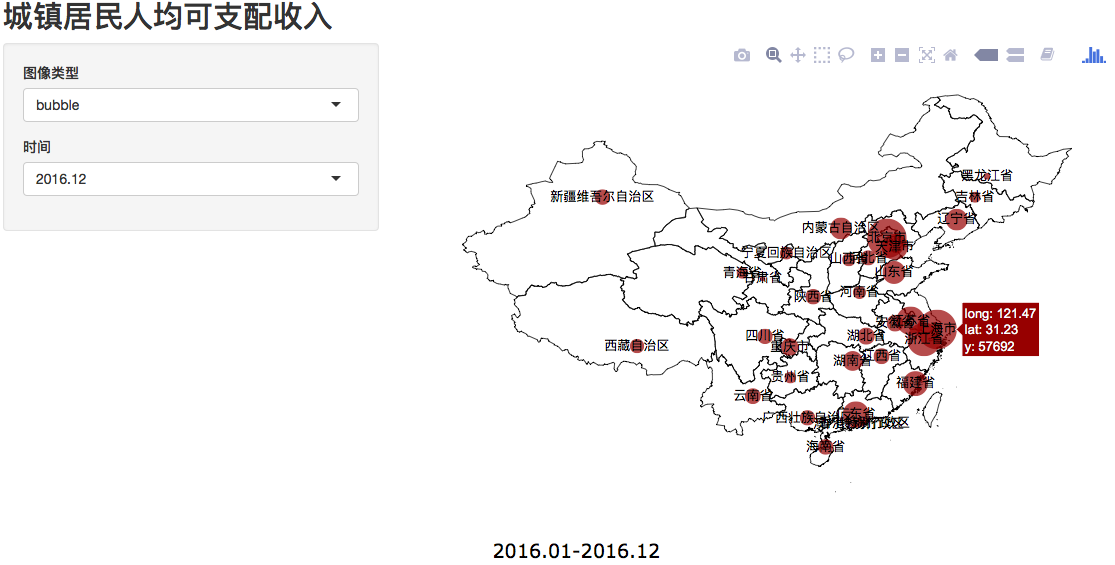
\includegraphics[width=400pt]{fig4.png}
	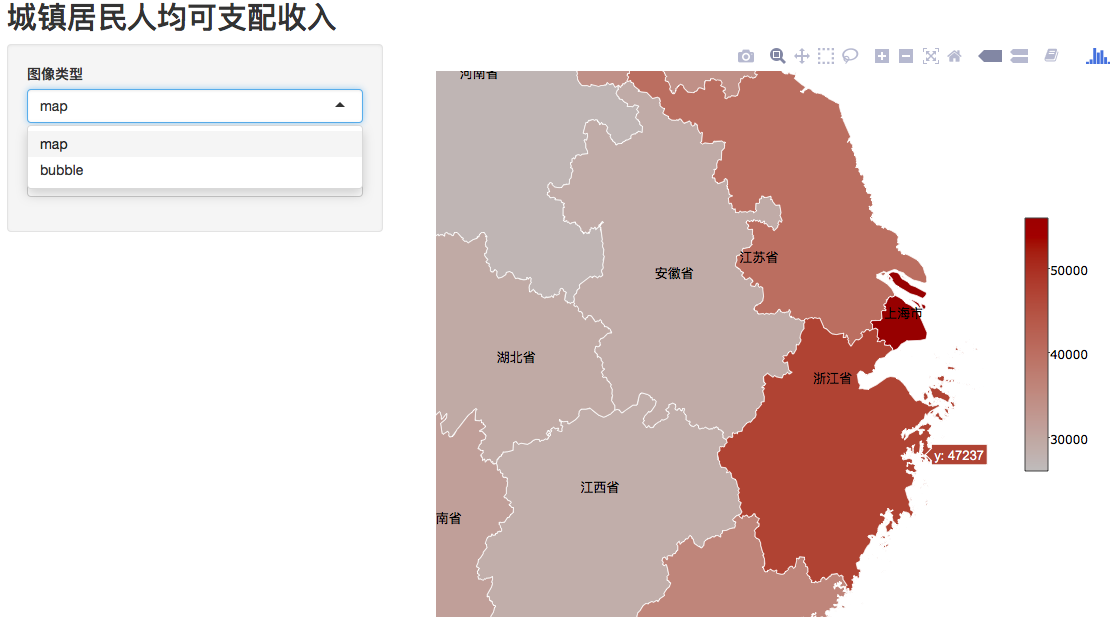
\includegraphics[width=400pt]{fig7.png}
	\caption{城镇居民家庭人均可支配收入地图}
\end{figure}

\begin{figure}[H]
	\centering
	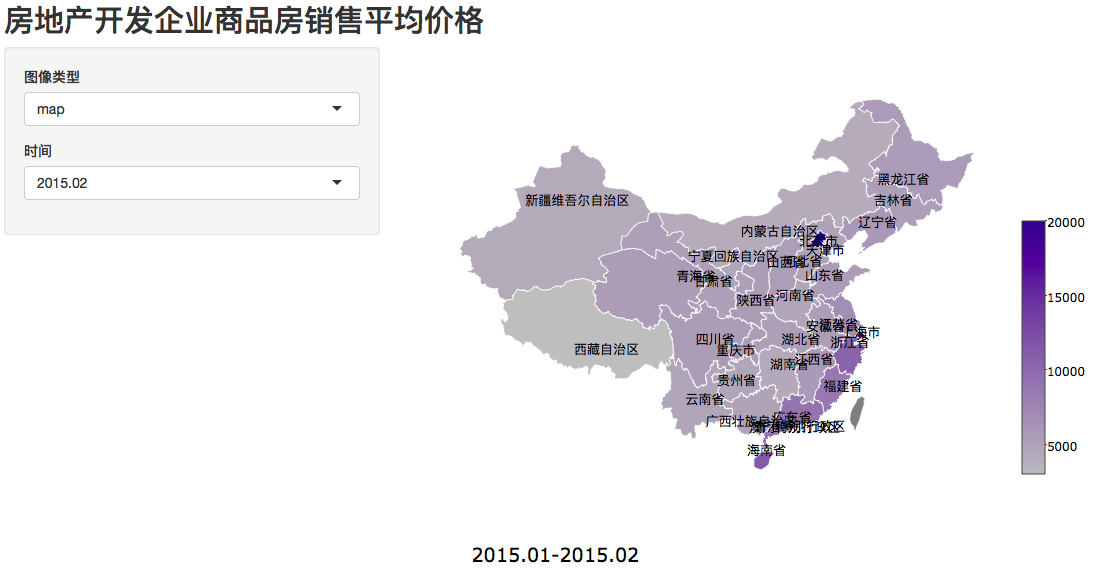
\includegraphics[width=400pt]{fig2.png}
	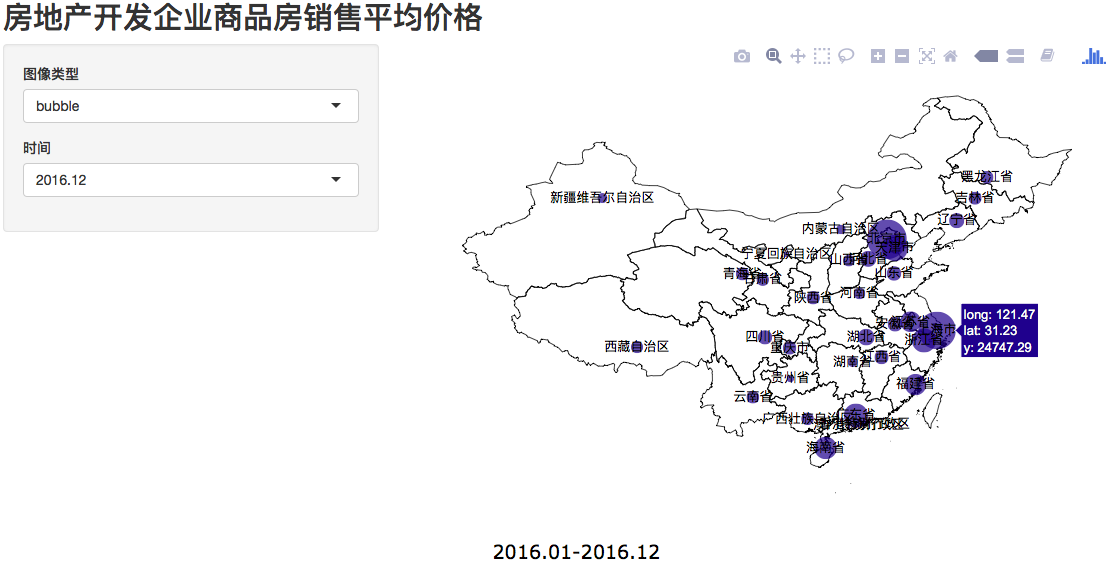
\includegraphics[width=400pt]{fig5.png}
	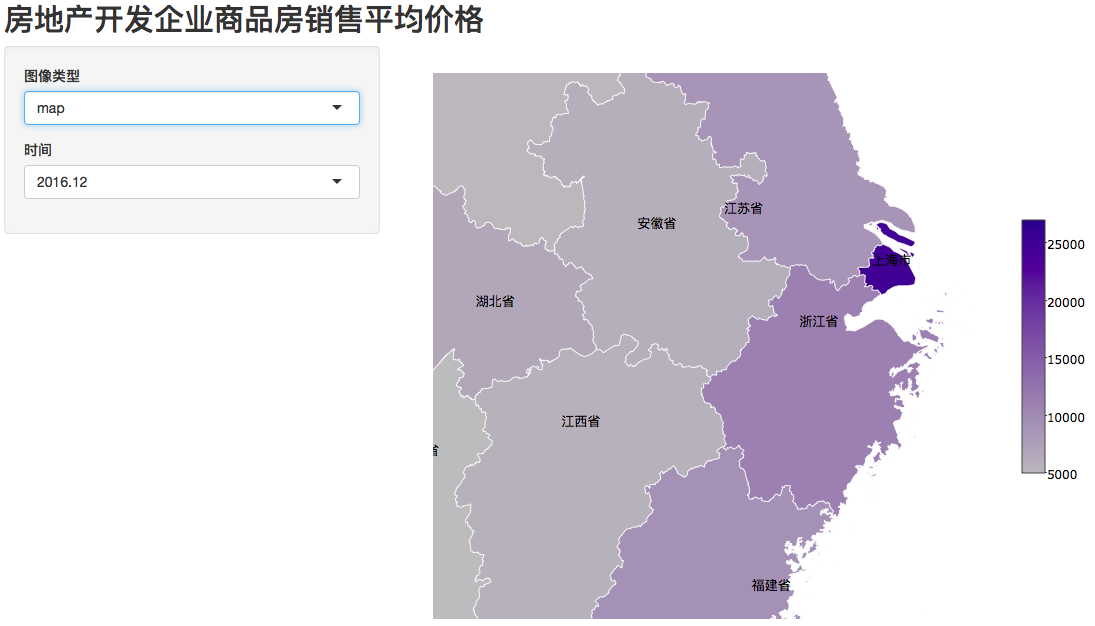
\includegraphics[width=400pt]{fig8.png}
	\caption{房地产开发企业商品房销售平均价格地图}
\end{figure}

\begin{figure}[H]
	\centering
	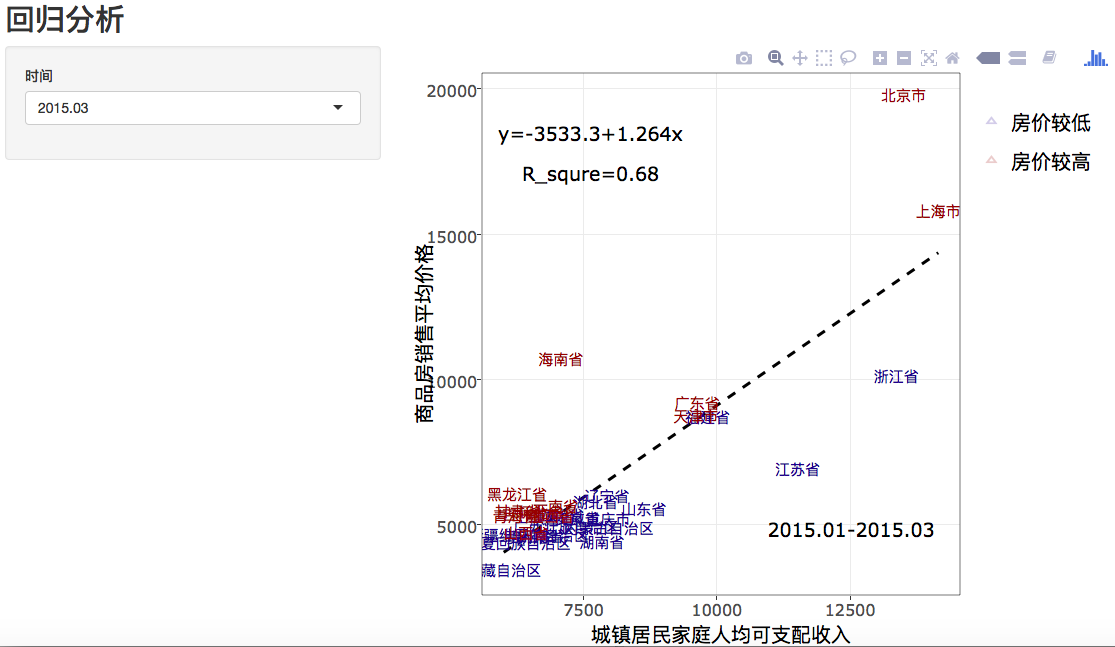
\includegraphics[width=400pt]{fig3.png}
	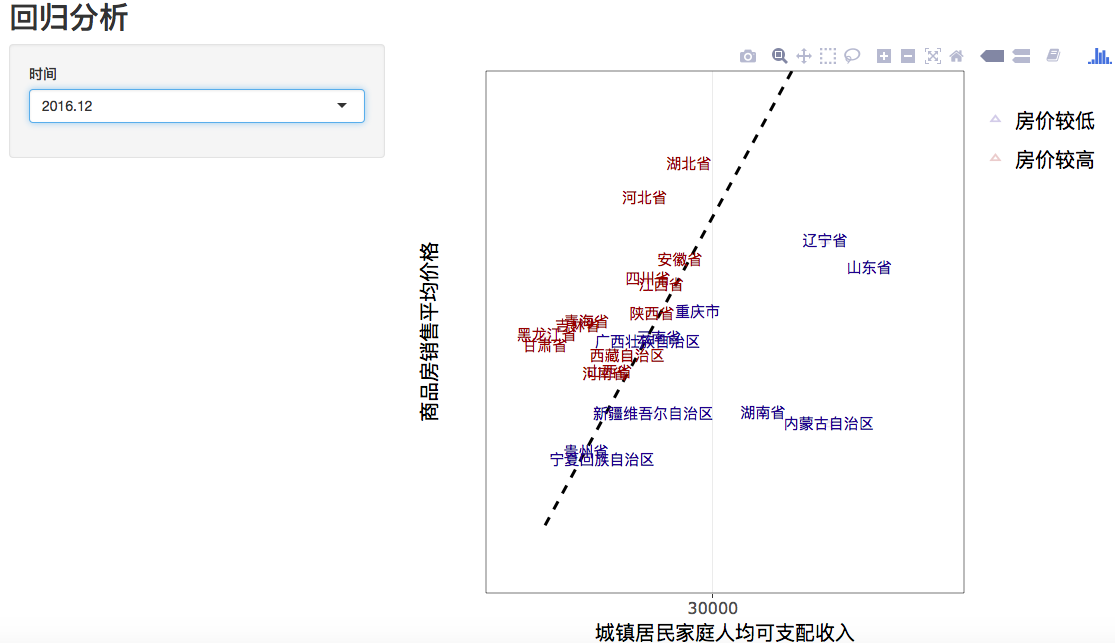
\includegraphics[width=400pt]{fig6.png}
	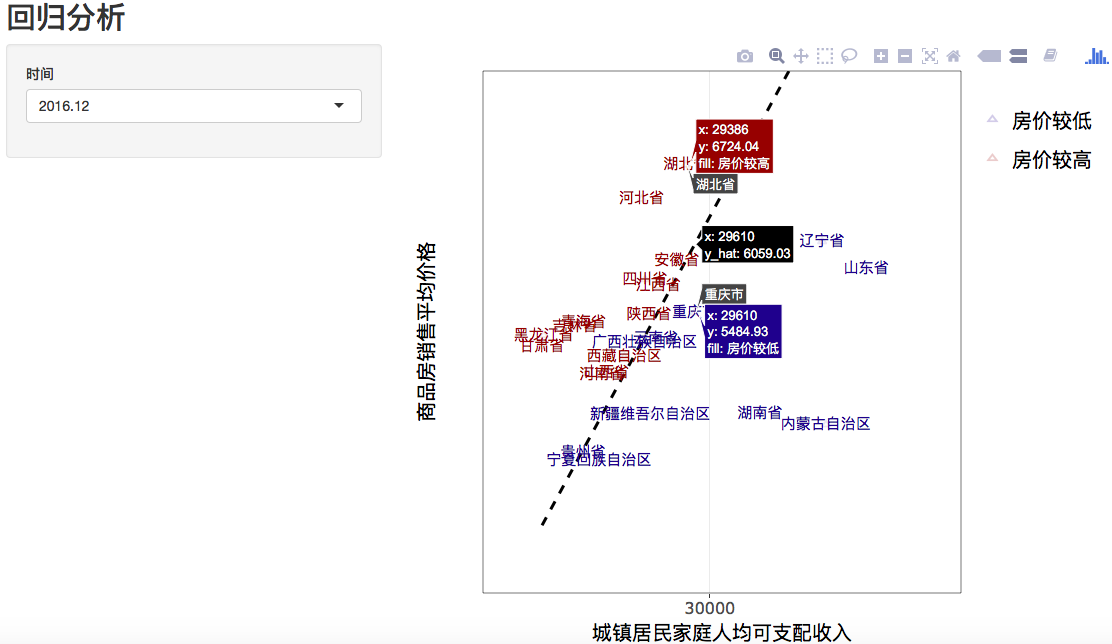
\includegraphics[width=400pt]{fig9.png}
	\caption{散点图与回归分析}
\end{figure}

\end{document}
